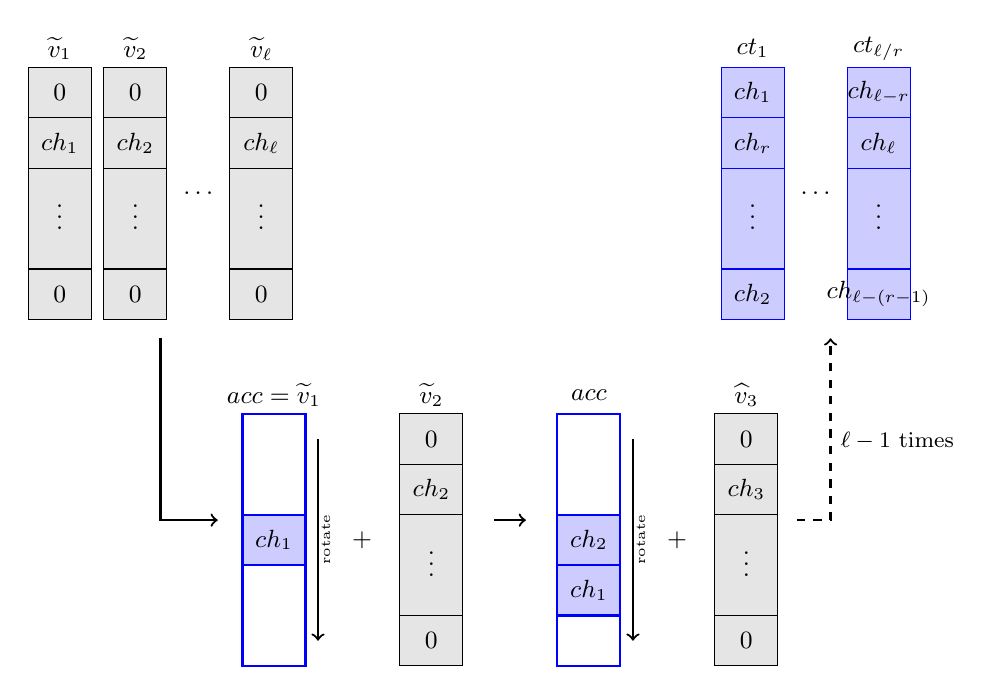
\begin{tikzpicture}[scale=0.8, every node/.style={font=\small}]
    
    % Original matrix wrapped in a scope with bounding box named "matrix" at the top
    \begin{scope}[local bounding box=matrix, shift={(-3cm,5.5cm)}]
        \draw[fill=gray!20, draw=black] (0,0) rectangle (1,4);
        \draw (0,0.8) -- (1,0.8);
        \draw (0,2.4) -- (1,2.4);
        \draw (0,3.2) -- (1,3.2);
        \node at (0.5,4.3) {$\widetilde{v}_1$};
        \node at (0.5,2.8) {$ch_1$};
        \node at (0.5,0.4) {$0$};
        \node at (0.5,3.6) {$0$};
        \node at (0.5,1.75) {$\vdots$};

        \draw[fill=gray!20, draw=black] (1.2,0) rectangle (2.2,4);
        \draw (1.2,0.8) -- (2.2,0.8);
        \draw (1.2,2.4) -- (2.2,2.4);
        \draw (1.2,3.2) -- (2.2,3.2);
        \node at (1.7,4.3) {$\widetilde{v}_2$};
        \node at (1.7,2.8) {$ch_2$};
        \node at (1.7,0.4) {$0$};
        \node at (1.7,3.6) {$0$};
        \node at (1.7,1.75) {$\vdots$};

        \node at (2.7,2) {$\dots$};

        \draw[fill=gray!20, draw=black] (3.2,0) rectangle (4.2,4);
        \draw (3.2,0.8) -- (4.2,0.8);
        \draw (3.2,2.4) -- (4.2,2.4);
        \draw (3.2,3.2) -- (4.2,3.2);
        \node at (3.7,4.3) {$\widetilde{v}_\ell$};
        \node at (3.7,2.8) {$ch_{\ell}$};
        \node at (3.7,0.4) {$0$};
        \node at (3.7,3.6) {$0$};
        \node at (3.7,1.75) {$\vdots$};
    \end{scope}

    % Sum of 2 ciphertexts block below the arrow
    \begin{scope}[local bounding box=horizontal, shift={(0.4cm,0cm)}]
        \begin{scope}[local bounding box=sumblock]
            % First ciphertext
            \draw[blue, thick] (0,0) rectangle (1,4);
            \draw[fill=blue!20, draw=blue, thick] (0,1.6) rectangle (1,2.4);
            \node at (0.5,4.3) {$acc = \widetilde{v}_1$};
            \node at (0.5,2) {$ch_1$};
            \draw[->,thick] (1.2,3.6) -- (1.2,0.4) node[midway,xshift=0.1cm ,rotate=90,font=\tiny] {rotate};

            % Plus sign
            \node at (1.9,2) {$+$};

            % Second ciphertext
            \draw[fill=gray!20, draw=black] (2.5,0) rectangle (3.5,4);
            \draw (2.5,0.8) -- (3.5,0.8);
            \draw (2.5,2.4) -- (3.5,2.4);
            \draw (2.5,3.2) -- (3.5,3.2);
            \node at (3,4.3) {$\widetilde{v}_2$};
            \node at (3,2.8) {$ch_2$};
            \node at (3,0.4) {$0$};
            \node at (3,3.6) {$0$};
            \node at (3,1.75) {$\vdots$};
        \end{scope}

        % Horizontal arrow between sum blocks
        \draw[->,thick] ([xshift=0.5cm]sumblock.east) -- ++(0.5,0);

        % Second sum block positioned horizontally next to the first
        \begin{scope}[local bounding box=sumblock2, shift={([xshift=1.5cm]sumblock.south east)}]
            % First ciphertext
            \draw[blue, thick] (0,0) rectangle (1,4);
            \draw[fill=blue!20, draw=blue, thick] (0,0.8) rectangle (1,2.4);
            \draw[blue, thick] (0,1.6) -- (1,1.6);
            \node at (0.5,4.3) {$acc$};
            \node at (0.5,2) {$ch_2$};
            \node at (0.5,1.2) {$ch_1$};
            \draw[->,thick] (1.2,3.6) -- (1.2,0.4) node[midway,xshift=0.1cm ,rotate=90,font=\tiny] {rotate};

            % Plus sign
            \node at (1.9,2) {$+$};

            % Second ciphertext
            \draw[fill=gray!20, draw=black] (2.5,0) rectangle (3.5,4);
            \draw (2.5,0.8) -- (3.5,0.8);
            \draw (2.5,2.4) -- (3.5,2.4);
            \draw (2.5,3.2) -- (3.5,3.2);
            \node at (3,4.3) {$\widehat{v}_3$};
            \node at (3,2.8) {$ch_3$};
            \node at (3,0.4) {$0$};
            \node at (3,3.6) {$0$};
            \node at (3,1.75) {$\vdots$};
        \end{scope}
    \end{scope}

    \draw[->,thick] ([yshift=-0.3cm]matrix.south) |- (horizontal.west);
    
    % Final result matrix
    \begin{scope}[local bounding box=return_matrix, shift={(8cm,5.5cm)}]
        \draw[fill=blue!20, draw=blue] (0,0) rectangle (1,4);
        \draw[blue] (0,0.8) -- (1,0.8);
        \draw[blue] (0,2.4) -- (1,2.4);
        \draw[blue] (0,3.2) -- (1,3.2);
        \node at (0.5,4.3) {$ct_1$};
        \node at (0.5,2.8) {$ch_r$};
        \node at (0.5,0.4) {$ch_2$};
        \node at (0.5,3.6) {$ch_1$};
        \node at (0.5,1.75) {$\vdots$};

        \node at (1.5,2) {$\dots$};

        \draw[fill=blue!20, draw=blue] (2,0) rectangle (3,4);
        \draw[blue] (2,0.8) -- (3,0.8);
        \draw[blue] (2,2.4) -- (3,2.4);
        \draw[blue] (2,3.2) -- (3,3.2);
        \node at (2.5,4.3) {$ct_{\ell/r}$};
        \node at (2.5,2.8) {$ch_{\ell}$};
        \node at (2.5,0.4) {$ch_{\ell-(r-1)}$};
        \node at (2.5,3.6) {$ch_{\ell-r}$};
        \node at (2.5,1.75) {$\vdots$};
    \end{scope}

    \draw[->,thick, dashed] ([xshift=0.3cm]horizontal.east) -| ([yshift=-0.3cm]return_matrix.south) node[midway, right, yshift=1cm] {\footnotesize $\ell-1$ times};

\end{tikzpicture}